\documentclass[11pt,a4paper,spanish]{book}
%\usepackage{estilo_unir}
\usepackage{biblatex}
\usepackage[utf8]{inputenc}
\usepackage{graphicx}
\graphicspath{ {./chapters/.images/} }
\usepackage{float}
\usepackage{hyperref}
\usepackage[utf8]{inputenc}

\addbibresource{referenceLib.bib}



\begin{document}
	%---------------------------
	%título del trabajo y autor
	%---------------------------
	\title{Reconocimiento y clasificación de emociones en la lengua no aprendidas}
	\author{Luisa Sánchez Avivar}
	%\date{d de mes de 2019}
	%\director{CiroRodríguez}
	%\nombreciudad{Lausanne}
	
	%---------------------------
	%marges
	%---------------------------
	%\usepackage[margin=1.9cm]{geometry}
	%---------------------------
	%---------------------------
	%---------------------------
	%---------------------------
	
	
	\mainmatter
	\chapter{Introducción}
	Desde hace años, el reconocimiento de emociones a través de la voz ha sido motivo de interés para la investigación, sin embargo siempre se ha estudiado sobre un mismo lenguaje debatiendo la habilidad de reconocer y clasificar las emociones oralmente expresadas. Esta habilidad ha sido respaldada por numerosos artículos donde se concluye que es posible distinguir e identificar entre al menos cuatro emociones básicas (felicidad, tristeza, tristeza, y enfado) a través de la voz (sin necesidad del procesamiento del lenguaje natural y por lo tanto de un contexto).
	
	Atendiendo al estudio de las emociones expresadas según la lengua existen estudios donde se demuestra que individuos de diferentes culturas pueden reconocer emociones básicas en diferentes niveles, pero es menos abundante la evidencia de un acuerdo en cómo las emociones básicas son reconocidas desde la expresión vocal de un interlocutor \cite{Pell2009a}
	Análogamente el debate del reconocimiento de emociones en un plano intercultural también se ha enfocado a través del estudio de los gestos faciales en conjunto con la expresión vocal, donde se concluye los factores sociales tienen un gran impacto, ya que la identificación de las emociones es más fácil para los miembros de la misma cultura que para los de otra distinta \cite{Pell2009a} y \cite{Pell2009}. A pesar de ello hay una gran carencia de comparativas con respecto a la voz donde se demuestre una sólida influencia cultural, sin embargo parece claro que las dimensiones socio culturales que engloban nuestras interacciones pueden tener un gran impacto en nuestra comunicación dentro de un marco emocional.
	
	La expresión de las emociones están íntimamente relacionadas con las propiedades fonéticas en el habla donde se observan señales y patrones para marcar contrastes lingüísticos en un idioma \cite{Pell2001} por lo tanto, los efectos del lenguaje en la comunicación emocional son evidentes al haber sido observadas y medidas, las variaciones en el rango tonal y la frecuencia para expresarlas, cambiando no sólo el tono si no también el patrón lingüístico asociado \cite{Davletcharova2015}. Por ejemplo la tristeza tiende a mostrarse con un tono notablemente bajo mientras que la felicidad, la sorpresa, o el enfado son producidas con un tono moderadamente alto. En general se esperaría que las expresiones de tristeza y enfado tiendan a marcar una mayor diferencia entre ellas y por lo tanto sean reconocidas con más precisión con independencia del lenguaje al estar situadas en los extremos (opuestos) del espectro.
	En literatura anterior \cite{Pell2011} se argumenta que las 6 emociones básicas felicidad, miedo, asco, sorpresa, enfado y tristeza) son exitósamente reconocidas desde la prosodia. Cabe destacar la diferencia entre prosodia y la calidad vocal, donde la primera se centra en características tales como la entonación, el estrés y el ritmo del habla mientras que la segunda se refiere al tono, energía y tempo \cite{Processing2015} . 
	
	Por otro lado tanto la proporción de consonantes y vocales (que hacen variar la presión de aire que se necesita) como el ratio de sílabas por palabra en cada idioma, caracterizan la expresión oral de las emociones. Existen muchos factores relacionados con el lenguaje como la morfología o la duración del estímulo que podrían ser un impacto en la decodificación de los matices en la señal vocal, tal y como explica en \cite{Chen2017}.
	
	Existe una clasificación dependiendo de la velocidad silábica en la expresión de dichos idiomas, sin embargo poco se conoce acerca de los efectos en las medidas respiratorias en el habla.Esta observación puede llevar a que se pregunte si en lenguajes tan dispares, las emociones expresadas mediante la voz puedan ser reconocidas desde el punto de vista del otro idioma.
	De nuevo, en \cite{Pell2009} se describen anómalas pseudo-manifestaciones semánticas (discurso sin sentido) que se asemejan a la lengua materna para expresar cada tipo de emoción. Aquí se evidencia claramente que la emoción de cada interlocutor puede ser reconocida con precisión desde la prosodia independientemente del contexto semántico. Además argumenta que el significado emocional en la voz se transmite por cambios en diferentes parámetros acústicos como el tono, la intensidad, la duración, el ritmo y distintos aspectos de la calidad de la voz.
	
	Finalmente, obtener datos necesarios de la extracción de características es un problema porque apenas cubre el amplio espectro emocional que hoy conocemos. C.Bakir y M.Yuzkat \cite{BAKIR2018} proponen un modelo híbrido para clasificar cinco emociones básicas en el lenguaje turco donde combinan SVM y GMM y aplicando antes MFCC y MFDWC para la extracción de características.
	
	
	
	
	\chapter{Estado del Arte}
	\section{Contexto}
	El objetivo del reconocimiento de emociones en el habla (a partir de ahora, referido como  SER, \emph{Speech Emotion Recognition} por sus siglas en inglés) es reconocer el trasfondo emocional del mensaje a través de la voz. Esta manifestación sonora posee factores clave para la comunicación humana que ayudan en su interacción sin alterar el contexto del mensaje.\\
	Normalmente estos estudios se llevan a cabo en un único lenguaje, lo que en el caso que nos acontece, se traduciría como el reconocimiento de emociones llevado a cabo en la lengua materna; Mientras este ejercicio puede llegar a ser intuitivo, distinguir las mismas emociones en la lengua extranjera supone un reto ya que implicaría importantes matices culturales. Por ejemplo, no sería lo mismo entender qué emociones intenta expresar un italo parlante desde el punto de vista de una persona que entiende el español (ambas lenguas latinas), que comprender las mismas emociones del discurso desde un germano hablante. Así bien, es importante definir qué idioma se está reconociendo y desde cuál, por lo que analizar las raíces lingüísticas y fonéticas de los idiomas a estudiar es esencial. 
	
	El proceso de la clasificación emocional en el lenguaje, consiste habitualmente, en tres partes: Procesamiento de la señal, que aplica filtros de audio a la señal original; Extracción de características, el cual es un punto esencial en esta modalidad ya que necesita enfatizar el contenido emocional sin depender del contexto lingüístico; Y por último, la clasificación, que será la encargada de mapear el conjunto de características extraídas anteriormente con las emociones etiquetadas que hayamos definido. Seguidamente se ofrece una revisión más detallada de estas etapas.
	
	\section{Extracción de Características}
	La extracción de características es una de las secciones más importantes en el reconocimiento de emociones a través de la voz debido a la ambigüedad de las características y la variedad vocal. La extracción de características es el paso principal en el procesamiento del diálogo (speech), y se lleva a cabo para centrarse en la información contenida en la señal y mejorar el grado de similitud y/o diferenciación entre las clases.\cite{Hellbernd2016} Hasta ahora, por lo general hay dos enfoques principales  con respecto al tipo de características usadas en SER:\\
	Los rasgos prosódicos, los cuales extraen información de la prosodia, en concreto, tono, energía y duración, y por otro lado, las características del tracto vocal que normalmente indican la distribución de la energía en la frecuencia del rango vocal (conocidos como Coeficientes Cepstrales).
	La mayoría de los estudios centrados en SER usan rasgos espectrales como la información extraída del tracto vocal, lo que supone obtener la información derivada del espectro de la señal de la voz y se usan para modelar los patrones de entonación y frecuencia del hablante\cite{Langari2020}.\\
	
	Comunmente las técnicas de extracción de características más usadas son 
	MFCC, LPC, LPCC y DWT. A continuación se ofrece una breve explicación de cada una de estas técnicas analizando sus puntos fuertes y débiles.\cite{Rashid2018} El objetivo no es entrar demasiado en detalle, si no dar una guía para entender la importancia de cada unos de los algoritmos para la extracción de características en el uso de SER.\hfill \break
	
	Los \textbf{Coeficientes Cepstrales en la escala de Mel} (MFCC, \emph{Mel Frecuency Cepstral Coefficients}), se basa en la desintegración de la señal para tener como resultado un resumen de las características que la forman. La obtención de este conjunto de valores numéricos se basa por un lado, en el rango de frecuencias de Mel, el cual consiste en una adaptación de frecuencias de la señal a aquellas más fácilmente percibidas por el oído humano, y por lo otro lado, la separación de frecuencias mediante \emph{Cepstrum} que divide la señal en dos bandas de frecuencias, baja (correspondientes a los fonemas producidos por el tracto vocal) y alta (correspondientes a la excitación de las cuerdas vocales). Debido a esto, encapsula la mayor parte de energía proveniente del sonido que es generado por humanos, por lo que es frecuentemente usada y sugerida para identificar palabras monosilábicas en un discurso.
	
	Los objetivos clave, serían:
	\begin{itemize}
		\item Eliminar la excitación del tracto vocal.
		\item Hacer independientes a las características extraídas.
		\item Ajuste a como los humanos percibimos el ruido y la frecuencia del sonido.
		\item Capturar la dinámica fonética, que definirá el contexto.
	\end{itemize}
	
	\begin{figure}[H]
		\centering
		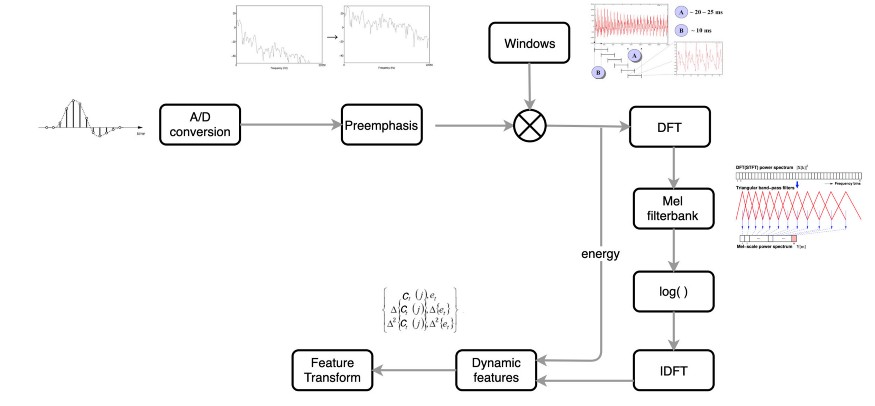
\includegraphics[scale=0.25]{MFCC_process.jpeg} 
		\caption{Proceso en la aplicación de MFCC en una señal.}
		\label{fig:mfcc_process}
	\end{figure}
	
	MFCC constituye una perfecta representación para el sonido cuando la fuente es estable y consistente. En \cite{Sarkania2013} implementa un sistema usando redes neuronales que se centra en el uso de MFCC como extracción de características y añade un filtro  de paso alto para reducir el ruido, consiguiendo una precisión de 93.38\% de media. En \cite{Wang2020} también se utiliza MFCC como método de extracción de características destacando especialmente su efectividad en SER combinada con espectogramas de Mel.\hfill \break
	
	
	Los \textbf{Coeficientes de Predicción Lineal} (LPC, \emph{Linear Prediction Coefficients}) se aplican para obtener el coeficiente de predicción lineal equivalente al tracto vocal reduciendo el mínimo error cuadrado entre la señal de audio dada como entrada y la estimada. Normalmente se usa para extraer las propiedades del tracto vocal ya que hace estimaciones bastante precisas de los parámetros en el habla, no obstante, es altamente sensible al ruido de cuantificación, por lo que demuestra no ser precisa cuando hay ruido de fondo y podría, y al igual que MFCC, no ser apropiada para la generalización.\hfill \break
	
	Los \textbf{Coeficientes Cepstrales con Predicción Lineal} (LPCC, \emph{Linear Prediction Cepstral Coefficient}) calcula una envolvente a LPC y luego hace una conversión a coeficientes cepstrales; Tiene una baja vulnerabilidad al ruido de fondo y mejora el ratio de error en comparación a LPC, pero sigue teniendo una gran sensibilidad al ruido de cuantificación.\hfill \break
	
	La \textbf{Transformada Wavelets} (DWT, \emph{Discrete Wavelet Transform}) descompone la señal en grupos de funciones básicas llamadas wavelets. La Transformada de Wavelet discreta es una extensión de esta donde mejora dicho proceso de descomposición discretizando los parámetros de tiempo y frecuencia. Los parámetros de DWT contienen información de diferentes escalas de frecuencia, lo cual es importante porque supone una mejora en la información que se obtiene del diálogo en la correspondiente banda de frecuencia. A pesar de ello, los coeficientes de Wavelet presentan variaciones indeseadas en los límites ya que las señales de entrada son de una longitud finita.\hfill \break
	
	
	
	\section{Clasificación}
	Convencionalmente, el estudio de SER incluye el uso de diferentes tipos de clasificadores para distinguir entre emociones: Suport Vector Machines (SVNs) los cuales se han usado extensamente para el reconocimiento de emociones y pueden llegar a presentar un buen rendimiento en comparación con otros clasificadores tradicionales, el algoritmo K-NN es de los enfoques más simples, Hidden Markov Model(HMM)es a menudo utilizado para lidiar con los cambios temporales en la señal y por último, Gaussian Mixture Model (GMM) el cual es útil para representar las unidades de sonido en características acústicas %\cite{Farooq2020}.
	No obstante,en estudios más recientes, se han propuesto clasificadores basados en aprendizaje profundo y en redes neuronales densas (DNN, \emph{Deep Neural Network}) los cuales han superado a los enfoques tradicionales resultando ser más eficientes además de tener la capacidad de aprender las características emocionales en el reconocimiento de emociones a través del audio.
	
	\subsection{RNN}
	Las Redes Recurrentes Neuronales (RNN, \emph{Recurrent Neural Network}) son convenientes en tareas en las que los datos son procesados secuencialmente.
	Lee y Tashev \cite{Lee2015} afirman que los sistemas basados en simples redes neuronales densas no cubren el efecto contextual a largo plazo para interpretar las emociones en el diálogo (esto es, la necesidad de un contexto emocional previo en la prosodia para mejorar la clasificación en el tramo que se está actualmente analizando) y resuelven este problema presentando un modelo basado en RNN. Por otro lado, W.Lim \cite{Lim2017} estudia el resultado de un sistema híbrido que usa CNN y RNN para clasificar emociones en una secuencia de audio, consiguiendo un 88.01\% de precisión.
	No obstante, los modelos RNN no son suficientes para representar el espectro emocional a lo largo de una conversación debido al problema de desvanecimiento de gradientes*.
	
	\subsection{LSTM}
	Los retos que presenta la clasificación de emociones en el habla, son comúnmente abordados a través de una red LSTM la cual es capaz de retener información de entradas anteriores en el tiempo y tener en cuenta dependencias temporales largas, ya que cada nodo es una célula de memoria. Esto a su vez, resuelve el problema de desvanecimiento de gradientes que presenta RNN.
	En el trabajo citado anteriormente \cite{Wang2020}, Wang propone un modelo dual LSTM para procesar dos espectogramas Mel simultáneamente, consiguiendo una precisión del 73.3\%. 
	Sin embargo este tipo de modelos no suelen implementarse como enfoque único, si no combinados con otro clasificador en una arquitectura más compleja. Por ejemplo en \cite{Lim2017} se lleva a cabo una comparación de tres  arquitecturas (CNN, LSTM y CNN distribuida en el tiempo) donde LSTM (utilizada de manera aislada) es la que puntúa más bajo.
	
	\subsection{CNN}
	La tendencia de los modelos DNN en este ámbito, es aprender características específicas desde varios métodos usados en el reconocimiento de emociones a través de la percepción acústica, en especial las redes neuronales convolucionales (CNN, \emph{Convolutional Neural Networks}) suponen una importante contribución en SER debido al uso de características significativas, y su uso en recientes estudios se ha incrementado a lo largo de los años.
	En \cite{Harar2017} describe un método que utiliza una arquitectura basada en redes convolucionales sin selección de características para distinguir únicamente entre tres emociones en alemán (usando Berlin Database Emotional Speech, la cual contiene 800 muestras de audio etiquetadas) consiguiendo una exactitud de 96.97\%. En \cite{AbdulQayyum2019} se presenta un modelo de redes convolucionales que no necesita de un preprocesado de la señal para una clasificación de emociones en el idioma inglés. Este utiliza la base de datos SAVEE, la cual contiene 480 muestras que distinguen entre 6 emociones, interpretadas por hombres y mujeres angloparlantes, donde obtiene finalmente un 81.63\% de precisión.
	
	
	\section{Valoración y Propuesta}
	En esta sección se valorarán las conclusiones que se extraigan del análisis previo sobre los distintas etapas correspondientes al desarrollo de un modelo para la clasificación de emociones en el habla. Los retos que plantea SER se han abordado anteriormente desde distintos enfoques, pero en su mayoría, para un único lenguaje. Las dificultades que presenta esta tarea en la lengua extranjera se deben principalmente a las posibles variaciones de aire para expresar la mismas emociones. Este mismo problema se plantea en una modalidad diferente pero bastante relacionada como es la transcripción de la voz a texto (ASR, \emph{Automatic Speech Recognition}), sin embargo estos estudios requieren un estudio más en profundidad de la fonética propia de cada lenguaje.
	
	Los trabajos de Pell se han centrado durante años en el análisis de la prosodia a través de los idiomas. A pesar de su antigüedad y que no entra demasiado en detalles técnicos, merece la pena mencionar que en \cite{Pell2008} lleva a cabo un estudio comparativo entre la detección emocional de la prosodia en la lengua materna y la extranjera, concluyendo que el proceso para entender las emociones vocales en una lengua no aprendida, implica una mayor exposición a esta para familiarizarse con señales prosódicas correspondientes a significados subyacentes.
	
	En la extracción de características el uso de MFCC ha sido ampliamente escogido al reportar resultados más elevados en comparación con otros métodos, mientras que en la sección donde se discuten los diversons métodos de clasificación usados en SER, vemos que CNN tiene mayor preferencia en la literatura, sin despreciar el uso de modelos basados en una combinación entre CNN y LSTM.\hfill \break
	El uso de CNN se ha vuelto cada vez más popular, especialmente en el procesamiento de imágenes, debido a que la principal ventaja que ofrecen en comparación con otras arquitecturas, es la habilidad de detectar características relevantes sin supervisión, a la vez que son computacionalmente eficientes.
	Ahora bien, el problema en el que se desarrolla en este trabajo gira en torno al procesamiento del audio, entonces, ¿cómo se pueden aprovechar las ventajas que provee CNN en este ámbito?
	
	No olvidemos que el tipo de dato con el que se trabajará principalmente serán señales, concretamente, de audio. En las señales de audio hay una cierta presión de aire que varía con respecto al tiempo, y al muestrearlas en un determinado rango de frecuencia, obtendríamos algo como lo siguiente:
	
	\begin{figure}[H]
		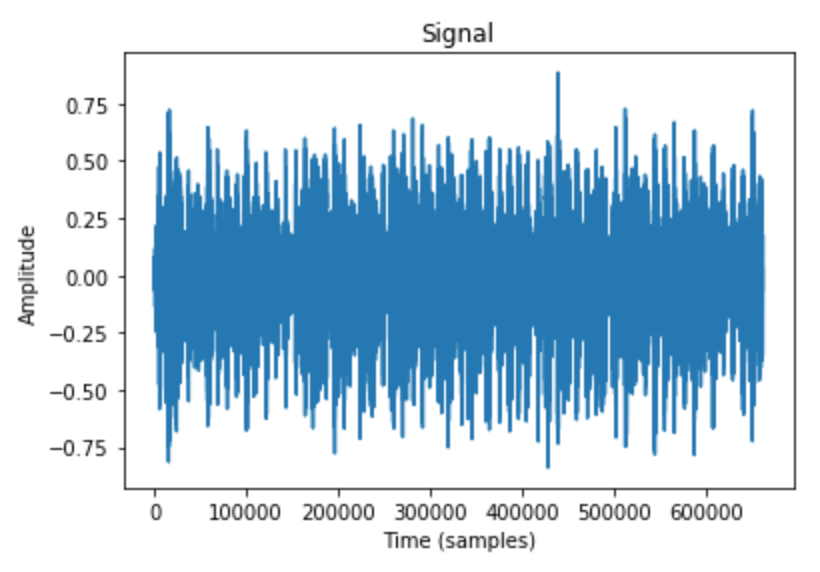
\includegraphics[scale=0.4]{waveform.png}
		\caption{waveform de una señal de audio}
	\end{figure}
	
	Esto que vemos es una representación digital de la onda, también llamada \emph{waveform}, de manera que ahora puede ser interpretada y analizada fácilmente.\hfill \break
	El siguiente punto que deberíamos atender, sería preguntarnos cómo extraer características relevantes de esta representación, y para ello se hace obvio pensar en la Transformada de Fourier (FFT \emph{Fast Fourier Transform}), la cual nos permite analizar la cantidad de frecuencia contenida en una señal. La Transformada de Fourier transforma la señal de un dominio de tiempo a un dominio de frencuencia, y el resultado de esta transformación se denomina espectro. \\
	Sin embargo el problema viene cuando en las señales de audio (que son el tipo de señales con las que queremos trabajar), la cantidad de frecuencia varía en el tiempo, por lo que FFT es insuficiente al no poder representar en el espectro resultante esta variación de la señal en el tiempo. La Transformada de Fourier en tiempo reducido, (\emph{short-time Fast Fourier Transform}) resuelve este problema calculando la FFT en segmentos (ventanas de tiempo) superpuestos de la señal. Lo que finalmente obtenemos se denomina \textbf{espectograma}.
	
	\begin{figure}[H]
		\centering
		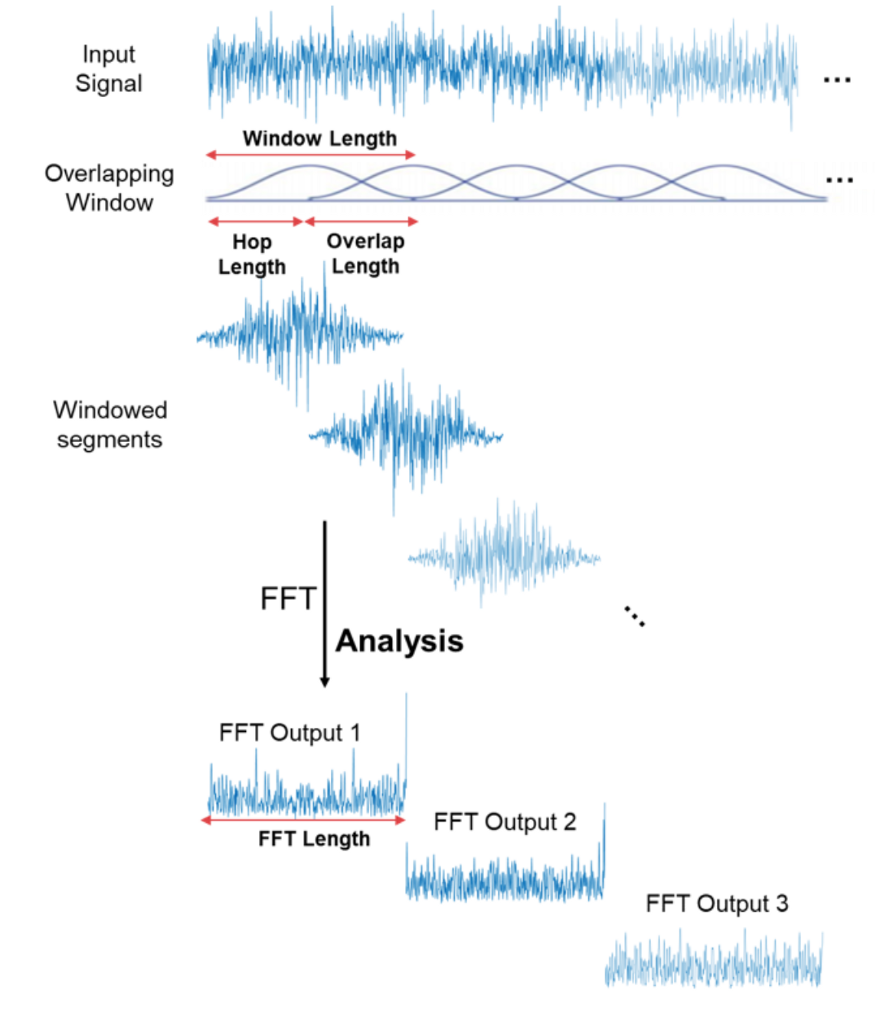
\includegraphics[scale=0.25]{processFFT.png} 
		\caption{Proceso del uso de FFT en una señal. Fuente: \href{https://www.mathworks.com/help/dsp/ref/dsp.stft.html}{Mathworks}}
	\end{figure} 
	
	
	Este espectograma puede ser entendido como una representación tridimensional de la señal donde sus características (tiempo, frecuencia y amplitud de la distribución de energía) pueden ser observadas de manera muy visual. Cuando este espectograma se computa, el eje X representa el tiempo, el eje Y representa la frecuencia, que es convertida a una escala logarítmica; En cuanto a la gama de colores que se utiliza, es para simbolizar la variación de energía expresada (medida decibelios), donde los tonos más oscuros indican unos valores de energía más altos, y viceversa.
	
	\begin{figure}[h]
		\centering
		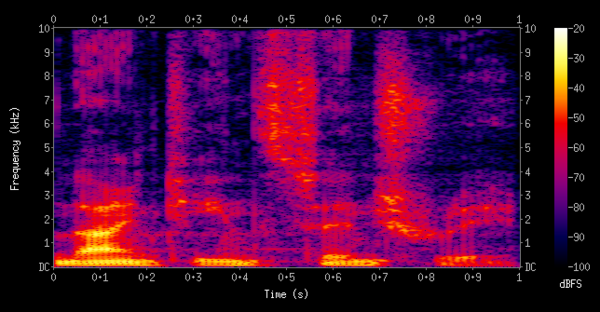
\includegraphics[scale=0.3]{spectogram.png} 
		\caption{Espectograma de una muestra aleatoria. Fuente: \href{https://es.other.wiki/wiki/Spectrogram}{Wiki}}
	\end{figure}
	
	La respuesta a por qué las frecuencias son convertidas a una escala logarítmica es sencillamente porque los humanos no percibimos las frecuencias en una escala lineal \cite{Varshney}, es decir, nuestra habilidad para distinguir entre frecuencias fluctúa a lo largo del rango en el que somos capaces de percibir\cite{StevensVolkmann}. Es por ello que el rango donde se mueve nuestro espectograma, se adapta a lo que se llama \textbf{escala de Mel}, en la cual los armónicos se observan equidistantes, reduciendo como resultado las variantes acústicas que no son significativas.\\
	
		Finalmente nos queda entender el concepto de \emph{Cepstrum} o coeficientes cepstrales, y para ello debemos entender como el sonido (respecto a la articulación de palabras) es producido. Técnicamente, esta producción del sonido en nuestra anatomía se definiría como la combinación de las vibraciones producidas por las cuerdas vocales con las vibraciones producidas por la resonancia del tracto vocal. Nuestras articulaciones controlan la forma del tracto vocal, por lo que la forma de onda (\emph{waveform}) de la voz será reprimida o amplificada a diferentes frecuencias por la forma de nuestro tracto vocal.\\
	El papel de Cepstrum es la separación de frecuencias en el algoritmo de MFCC, atendiendo a como los sonidos son producidos siguiendo un modelo anatómico, de manera que cuando es computado separa la señal de voz y la resonancia del tracto vocal. En \ref{fig:mfcc_process} observamos el paso IDFT, donde tras ajustar la señal a la escala de Mel, se calcula una variante de FFT (\emph{Inverse Discrete Fourier Transform}) y se obtienen los \textbf{coeficientes de MFCC}.
	
	\begin{figure}[h]
		\centering
		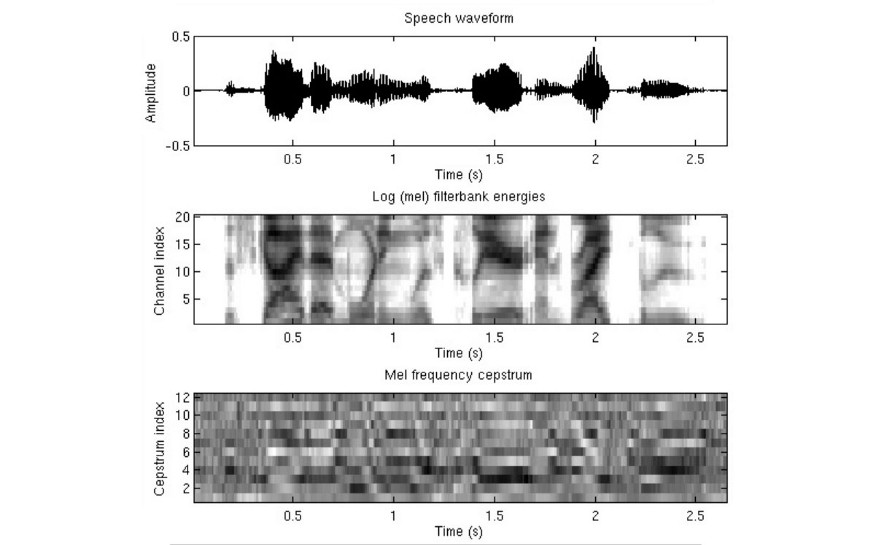
\includegraphics[scale=0.3]{waveform_process.jpeg} 
		\caption{Visualización de los coeficientes cepstrales de una muestra aleatoria. Fuente: \href{https://www.ee.columbia.edu/~stanchen/spring16/e6870/slides/lecture3.pdf}{Columbia University}}
	\end{figure}
	
	Dado que hemos convertido una señal de audio en una imagen, ahora se podrá proceder a usar un modelo basado en redes convolucionales, aprovechando sus ventajas en el campo donde mejor rendimiento reporta: el procesamiento de imágenes.
	
	\printbibliography
	
\end{document}


















